\large{
\section{Planarità}
\begin{figure}[!htb]
	\begin{center}
		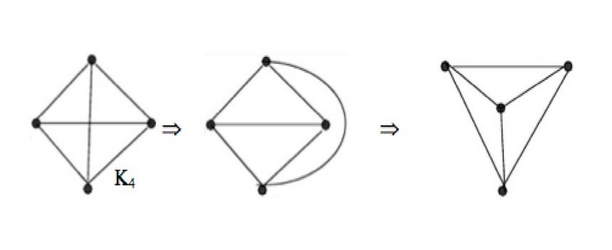
\includegraphics[width=1 \linewidth]{figure/planarita}
	\end{center}
	\caption{trasformazione del disegno di un grafo in un disegno planare \label{fig:planarita}}
\end{figure}
Data la definizione di grafo nel capitolo dedicato alle definizioni preliminari è necessario, ai fini di una introduzione al mondo della teoria dei grafi per ciò che concerne i grafi clusterizzati, enunciare la definizione di grafo planare.\\
Un grafo\textbf{ planare} $G$, come mostrato nella \figurename~\ref{fig:planarita}, è definito come un grafo tale che il suo disegno $\tau(G)$ può essere raffigurato in un piano in modo che non si abbiano archi che si intersecano tra loro. È facile da intuire che non tutti i grafi sono planari e se ne riportano due famosi esempi in \textbf{\figurename~\ref{fig:kuratowski}}. In particolare questi due grafi sono chiamati anche grafi di Kuratowski mediante i quali si può dare la definizione di grafo planare come enunciato del \textit{\textbf{Teorema di Kuratowski}}:
\begin{center}
	\textit{Un grafo è planare \textit{se e solo se} non contiene alcun sottografo che sia una espansione di $K_5 $ o una espansione di $K_{3,3}$\\}
\end{center}
\begin{figure}[!htb]
	\begin{center}
		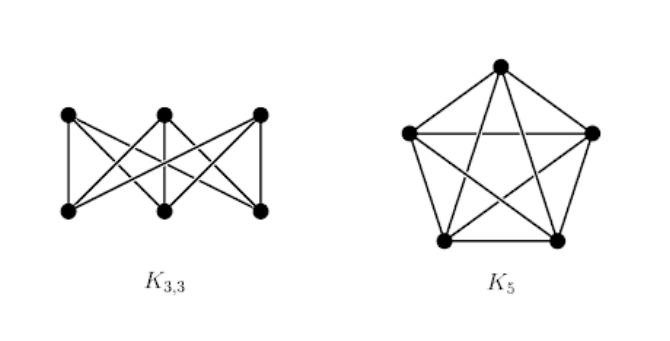
\includegraphics[width=0.9 \linewidth]{figure/kuratowski}
	\end{center}
	\caption{grafi di Kuratowski \label{fig:kuratowski}}
\end{figure}
Si ricorda inoltre che se un grafo è planare allora ammette un disegno planare $\tau(G)$. Dando un altra definizione si può evidenziare che un disegno $\tau(G)$ è un disegno planare se ogni arco non interseca nulla eccetto i due vertici che connette. Si richiama ora all'algoritmo di Auslander e Parter del 1961.\\ 
Mediante questo algoritmo, del costo non lineare a livello di complessità computazionale ma uguale a $O(n^3)$, si è in grado di calcolare se un grafo in input è planare o meno mediante due fasi. Nella prima si decompone un grafo arbitrario nelle sue componenti biconnesse e nella seconda si tenta di planarizzare ogni componente connessa. Definito grafo planare è anche possibile formulare il seguente teorema
\begin{center}
	\textit{un grafo è planare se il suo disegno è sempre colorabile con 4 colori diversi}
\end{center}
La planarità è un punto chiave nella teoria dei grafi e definizione fondamentale per l'introduzione ai grafi clusterizzati.

\section{C-graph}
\begin{figure}[!htb]
	\begin{center}
		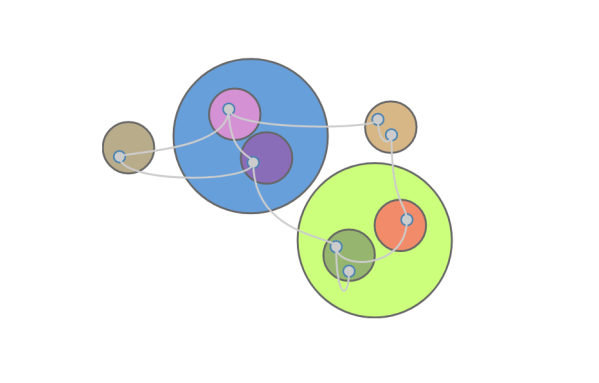
\includegraphics[width=0.9 \linewidth]{figure/cgraphGenerico}
	\end{center}
	\caption{esempio di grafo clusterizzato \label{fig:cgraphGenerico}}
\end{figure}
Un grafo clusterizzato (\textbf{c-graph}), di cui ne è un esempio la \textbf{\figurename~\ref{fig:cgraphGenerico}}, è definito come un grafo \textbf{planare} con una gerarchia ricorsiva definita sui suoi vertici. In altre parole un \textit{c-graph} C è definito come $$\textbf{C=<G,T>}$$ 
in cui:
\begin{itemize}
	\item\textbf{$G=(V,E)$} è un grafo planare, formato quindi da nodi e da archi le cui rappresentazioni non intersecano nulla se non il punto iniziale e finale, definito come \textit{underlying graph} di $C$;
	\item\textbf{$T$} è un albero radicato definito come \textit{inclusion tree} in cui l'insieme delle foglie di $T$ coincide con l'insieme dei nodi $V$ dell'underlying graph $G$ ed ogni nodo interno è rappresentato da un \textbf{cluster}.
\end{itemize}
Un cluster in informatica può essere definito come un insieme di oggetti simili spesso connessi tra loro a cui al suo interno può contenere altri sotto-cluster.
Nel caso specifico del termine si denota come un cluster potrà quindi contenere altri cluster al suo interno e/o nodi dell'insieme $V$ dell'Underlying graph $G$.
Un cluster essendo un nodo dell'albero di inclusione $T$ dovrà quindi avere una "conoscenza" del nodo precedente(genitore) e dei nodi successivi(figli) 

\section{clustered planarity}
Avendo definito la struttura di un grafo clusterizzato $C$ si può andare ad analizzare il comportamento per quanto concerne il disegno $\tau(C)$. 
Avendo inoltre definito l'underlying graph $G$come un grafo planare si devono fare delle considerazioni per quanto riguarda il disegno dell'intero grafo clusterizzato $C$(~\cite{feng1995planarity},~\cite{feng1997algorithms},~\cite{zbMATH05208230}).\\
Questo disegno $\tau(C)$ sarà un disegno planare clusterizzato \textbf{c-planar} se:\\
\begin{itemize}
	\item[(i)] ogni cluster è rappresentato da una singola regione del piano che contiene solo i suoi vertici e gli archi a cui essi sono collegati;
	\item[(ii)] definendo il perimetro del cluster come bordo del cluster, si ha che un disegno sarà planare se nessun bordo del disegno $\tau(C)$ si interseca con altri bordi di altri cluster;
	\item[(iii)] ogni arco si interseca con un cluster al più una volta;\\
\end{itemize}
Per ciò che concerne la teoria dell'informatica e dei grafi, i problemi relativi alla planarità e al disegno planare di grafi clusterizzati risultano essere ancora di grande importanza e oggetto di molte ricerche in quanto ancora non si è in grado di definire la complessità del decidere quando un generico grafo clusterizzato $C$ ammette un disegno planare clusterizzato $\tau(C)$.
In altre parole risulta essere un problema aperto quello di capire a quale classe di complessità appartiene il problema sopra definito, se in P o NP. La classe di complessità P consiste di tutti quei problemi di decisione che possono essere risolti con una macchina di Turing deterministica in un tempo che è polinomiale rispetto alla dimensione dei dati di ingresso. La classe \textbf{NP} consiste invece di tutti quei problemi di decisione le cui soluzioni positive possono essere verificate in tempo polinomiale avendo le giuste informazioni, o, equivalentemente, la cui soluzione può essere trovata in tempo polinomiale con una macchina di Turing non deterministica. Tutto questo poi richiama anche il problema del millennio \textit{P contro NP} che risulta ancora non risolto e che consiste nel capire se esistono problemi computazionali per cui è possibile "verificare" una soluzione in tempo polinomiale ma non è possibile "decidere", sempre in tempo polinomiale, se questa soluzione esiste. 
Si vuol precisare che le definizioni di macchina di Turing e di grammatiche di Chomsky non saranno date in questo lavoro poiché non necessarie ai fini dell'argomento trattato.
}